Dans la section suivantes, les résultats des différentes méthodes de commande sont comparés, ce qui permettra de conclure sur l'efficacité de chaque méthode.

\subsection{Rapidité et robustesse des algorithmes}

\subsection{Performances CPU et consommation de mémoire}

\underline{Rappel :} Le système d'exploitation du robot d'Artagnan est Ubuntu 22.04 version Server, tandis que les autres robots utilisent Ubuntu 22.04 version Desktop, ce qui explique les fortes différences de consommation, car la version Server est plus légère et consomme moins de ressources. Les configurations des robots ont été données précédemment (Tableau \ref{tab:config-robots}).

% Requires \usepackage{float} in the preamble for [H]
\begin{figure}[H]
    \centering
    \begin{subfigure}[t]{0.495\linewidth}
        \centering
        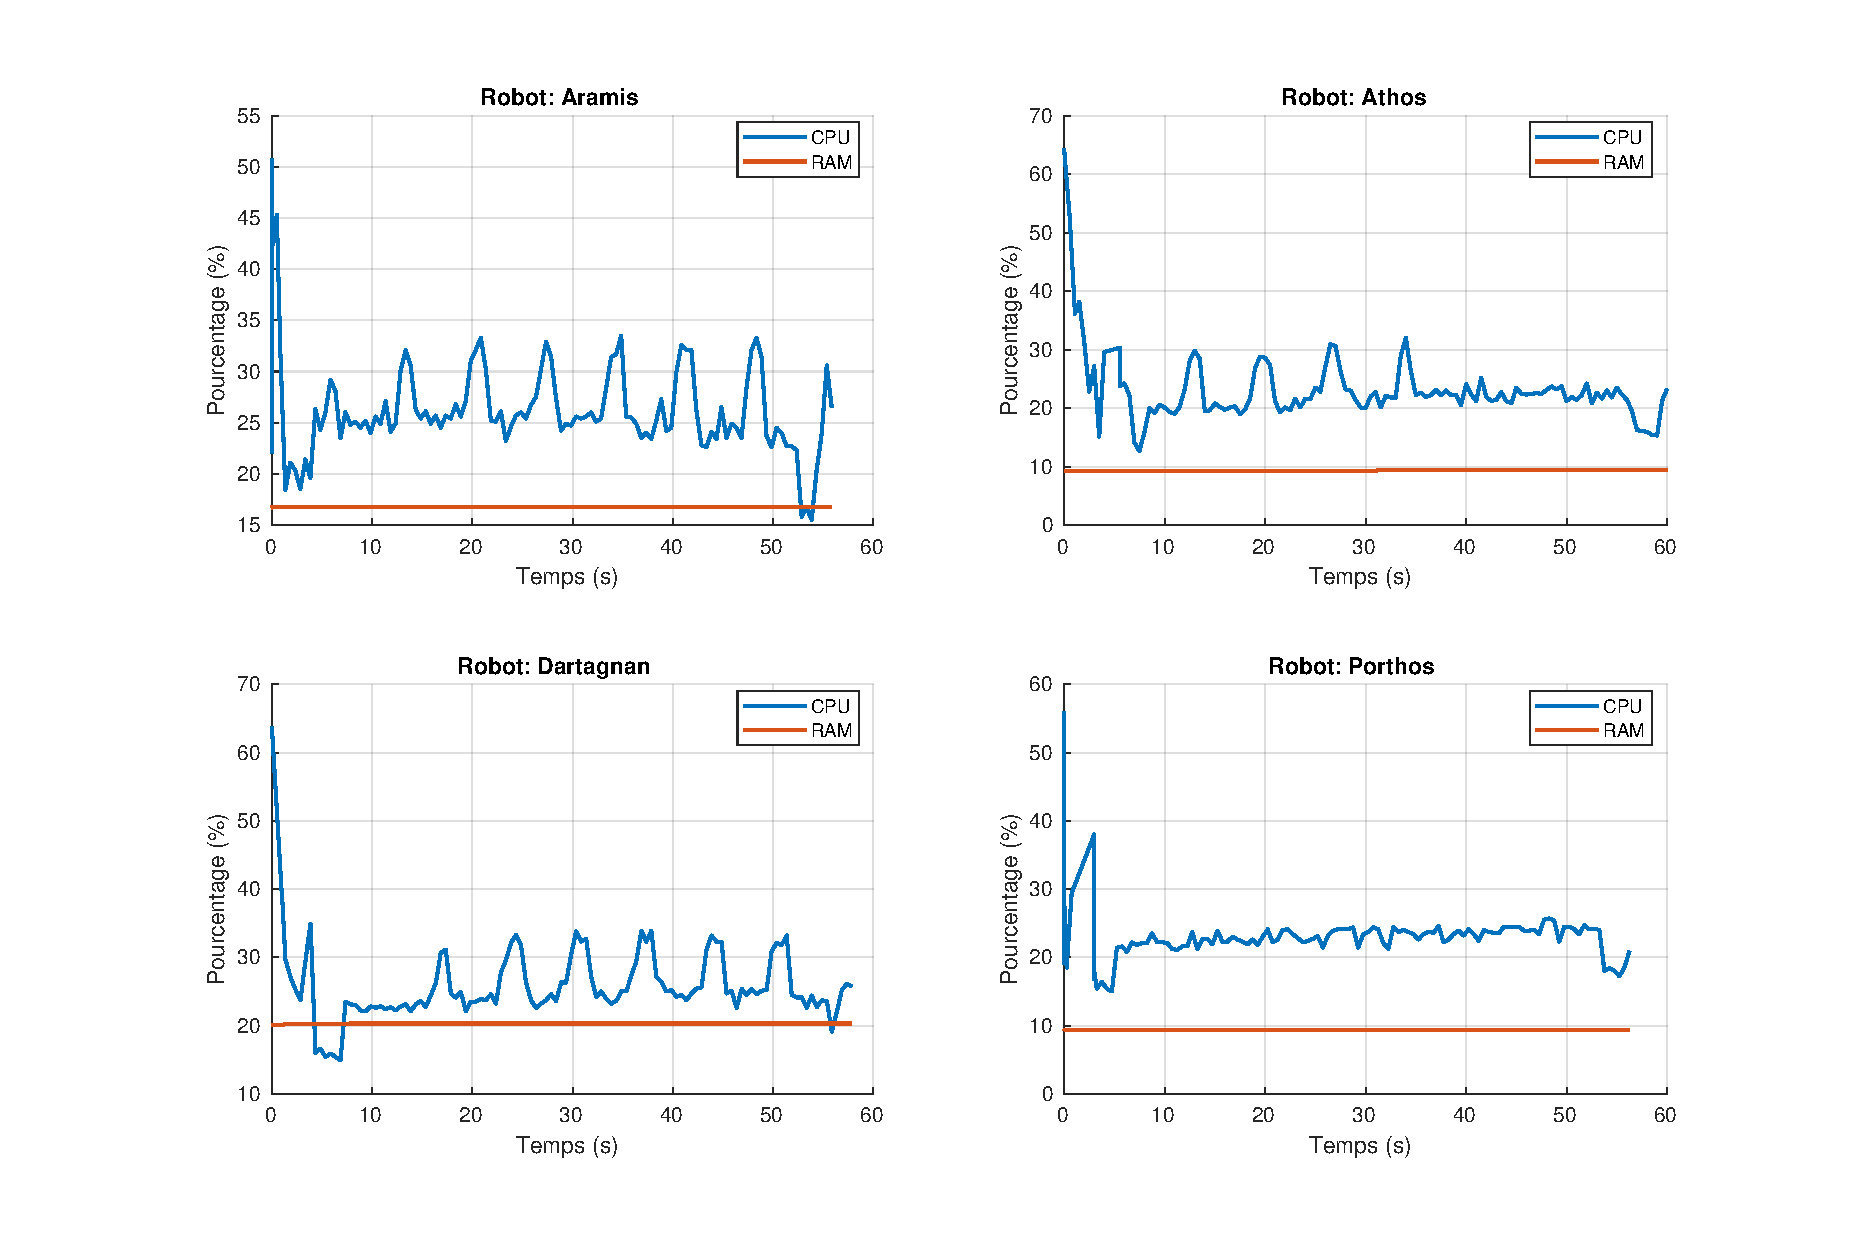
\includegraphics[width=\linewidth,height=6cm,keepaspectratio]{11-Résultats/pic/classic/cpu_ram.pdf}
        \caption{Méthode classique}
        \label{fig:cpu-ram-classic}
    \end{subfigure}%
    \begin{subfigure}[t]{0.495\linewidth}
        \centering
        
\includegraphics[width=\linewidth,height=6cm,keepaspectratio]{11-Résultats/pic/ev/cpu_ram.pdf}
        \caption{Méthode événementielle}
        \label{fig:cpu-ram-ev}
    \end{subfigure}

    \vspace{0.2em}

    \begin{subfigure}[t]{0.48\linewidth}
        \centering
        
\includegraphics[width=\linewidth,height=6cm,keepaspectratio]{11-Résultats/pic/pred/cpu_ram.pdf}
        \caption{Méthode prédictive}
        \label{fig:cpu-ram-pred}
    \end{subfigure}

    \caption{Utilisation CPU et RAM par robot}
    \label{fig:consommation-ram-robots}
\end{figure}



\begin{figure}[H]
    \centering
    \begin{subfigure}[t]{0.495\linewidth}
        \centering
        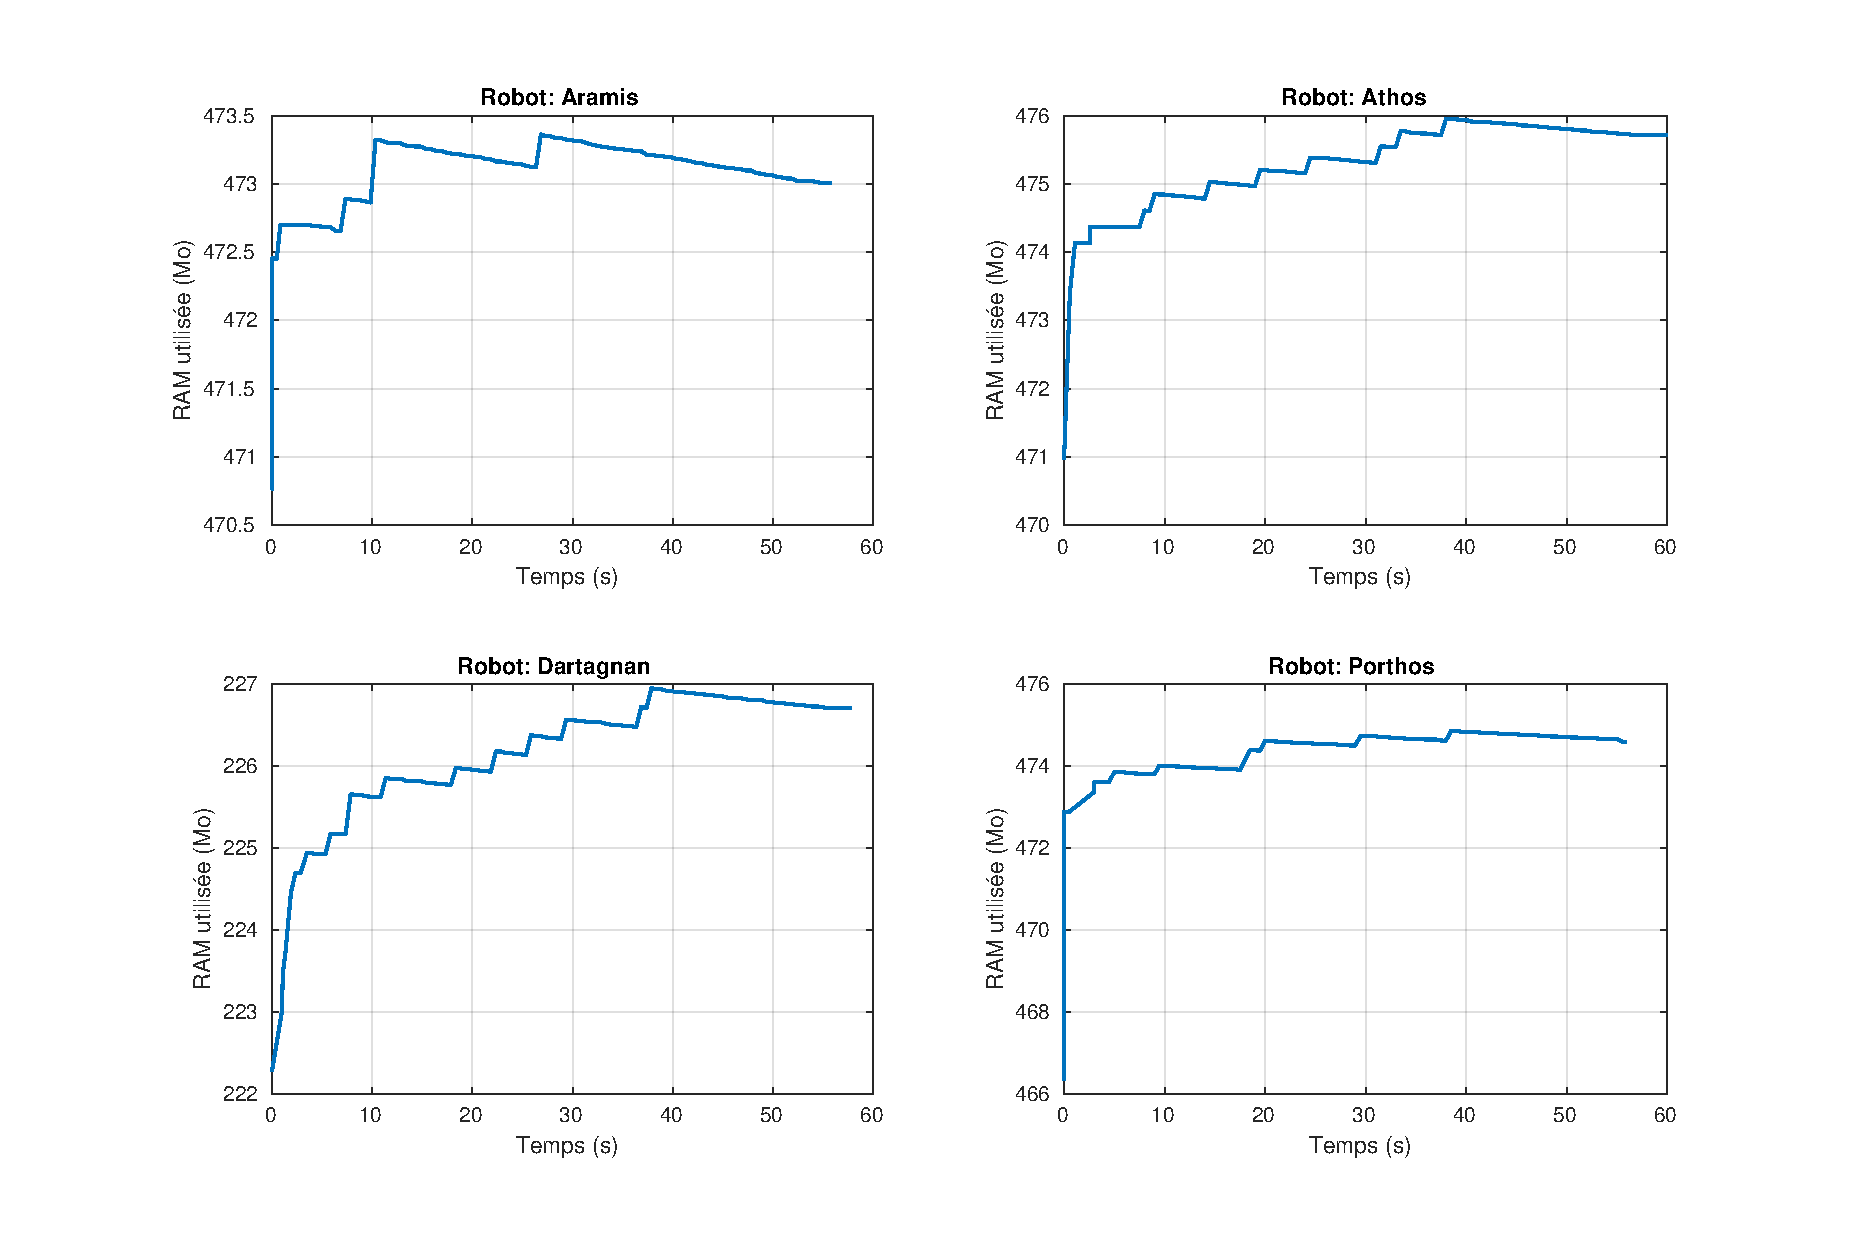
\includegraphics[width=\linewidth,height=6cm,keepaspectratio]{11-Résultats/pic/classic/ram_used.pdf}
        \caption{Méthode classique}
        \label{fig:ram-classic}
    \end{subfigure}%
    \begin{subfigure}[t]{0.495\linewidth}
        \centering
        
\includegraphics[width=\linewidth,height=6cm,keepaspectratio]{11-Résultats/pic/ev/ram_used.pdf}
        \caption{Méthode événementielle}
        \label{fig:ram-ev}
    \end{subfigure}

    \vspace{0.2em}

    \begin{subfigure}[t]{0.48\linewidth}
        \centering
        
\includegraphics[width=\linewidth,height=6cm,keepaspectratio]{11-Résultats/pic/pred/ram_used.pdf}
        \caption{Méthode prédictive}
        \label{fig:ram-pred}
    \end{subfigure}

    \caption{RAM par robot}
    \label{fig:ram-robots}
\end{figure}

Ces courbes permettent de visualiser que la quantité de RAM utilisés par les robots pour les trois méthodes est similaire. Pour ce qui est de l'utilisation CPU, elle est d'environ 20\% pour la méthode classique et événementielle, et légèrement inférieur pour la méthode prédictive, qui est d'environ 15\%, démontrant que la réduction des échanges d'informations entre les robots permet de réduire la charge CPU.
Il est toutefois possible de constater, hors du périmètre strict du projet, que le robot d'Artagnan, fonctionnant sous Ubuntu Server, présente une consommation de RAM environ deux fois plus faible que les autres robots.
